%! Author = maa
%! Date = 4/21/22

% Preamble
\documentclass[11pt]{article}

\usepackage[hidelinks]{hyperref}
\usepackage{csquotes}
\usepackage{pdfpages}
\title{Transcript}
\author{Matt Yan}

% Packages
\usepackage{amsmath}

% Document
\begin{document}

    \maketitle

    As explained in my personal statement, considering my over-all GPA,
    rather than the current program (General Mathematics) listed on the transcript,
    the school allows me to graduate with a B.Sc. in Math Specialization,
    which has stricter GAP requirements and a stricter course requirements consisting of more math courses.
    I have requested proof statements from the school of the degree change and completion,
    yet the school informs me that this won't show up on the transcript until late May 2022, after which
    the sping convocation of the University of Alberta is officially held,
    when I will receive a certification of my undergraduate degree.
    To that end, I have attached my correspondence with the advisor in the Science department of University of Alberta.

    Please also note the transcript is electronic but is officially requested from the University of Alberta.
    Alternatively, it can be viewed from the link below with my school email address syan4@ualberta.ca as the password,
    where more issuer and certification information can be seen:

    \href{https://learner.mycreds.ca/#/sharelink/af3520e0-ad1f-4714-bb4c-04e6eada9091/d0dceb4e-a2e5-4622-9760-6930b4b55315}{
        \tiny{https://learner.mycreds.ca/\#/sharelink/af3520e0-ad1f-4714-bb4c-04e6eada9091/d0dceb4e-a2e5-4622-9760-6930b4b55315}
    }

    \newpage
    \section*{Official Transcript}

    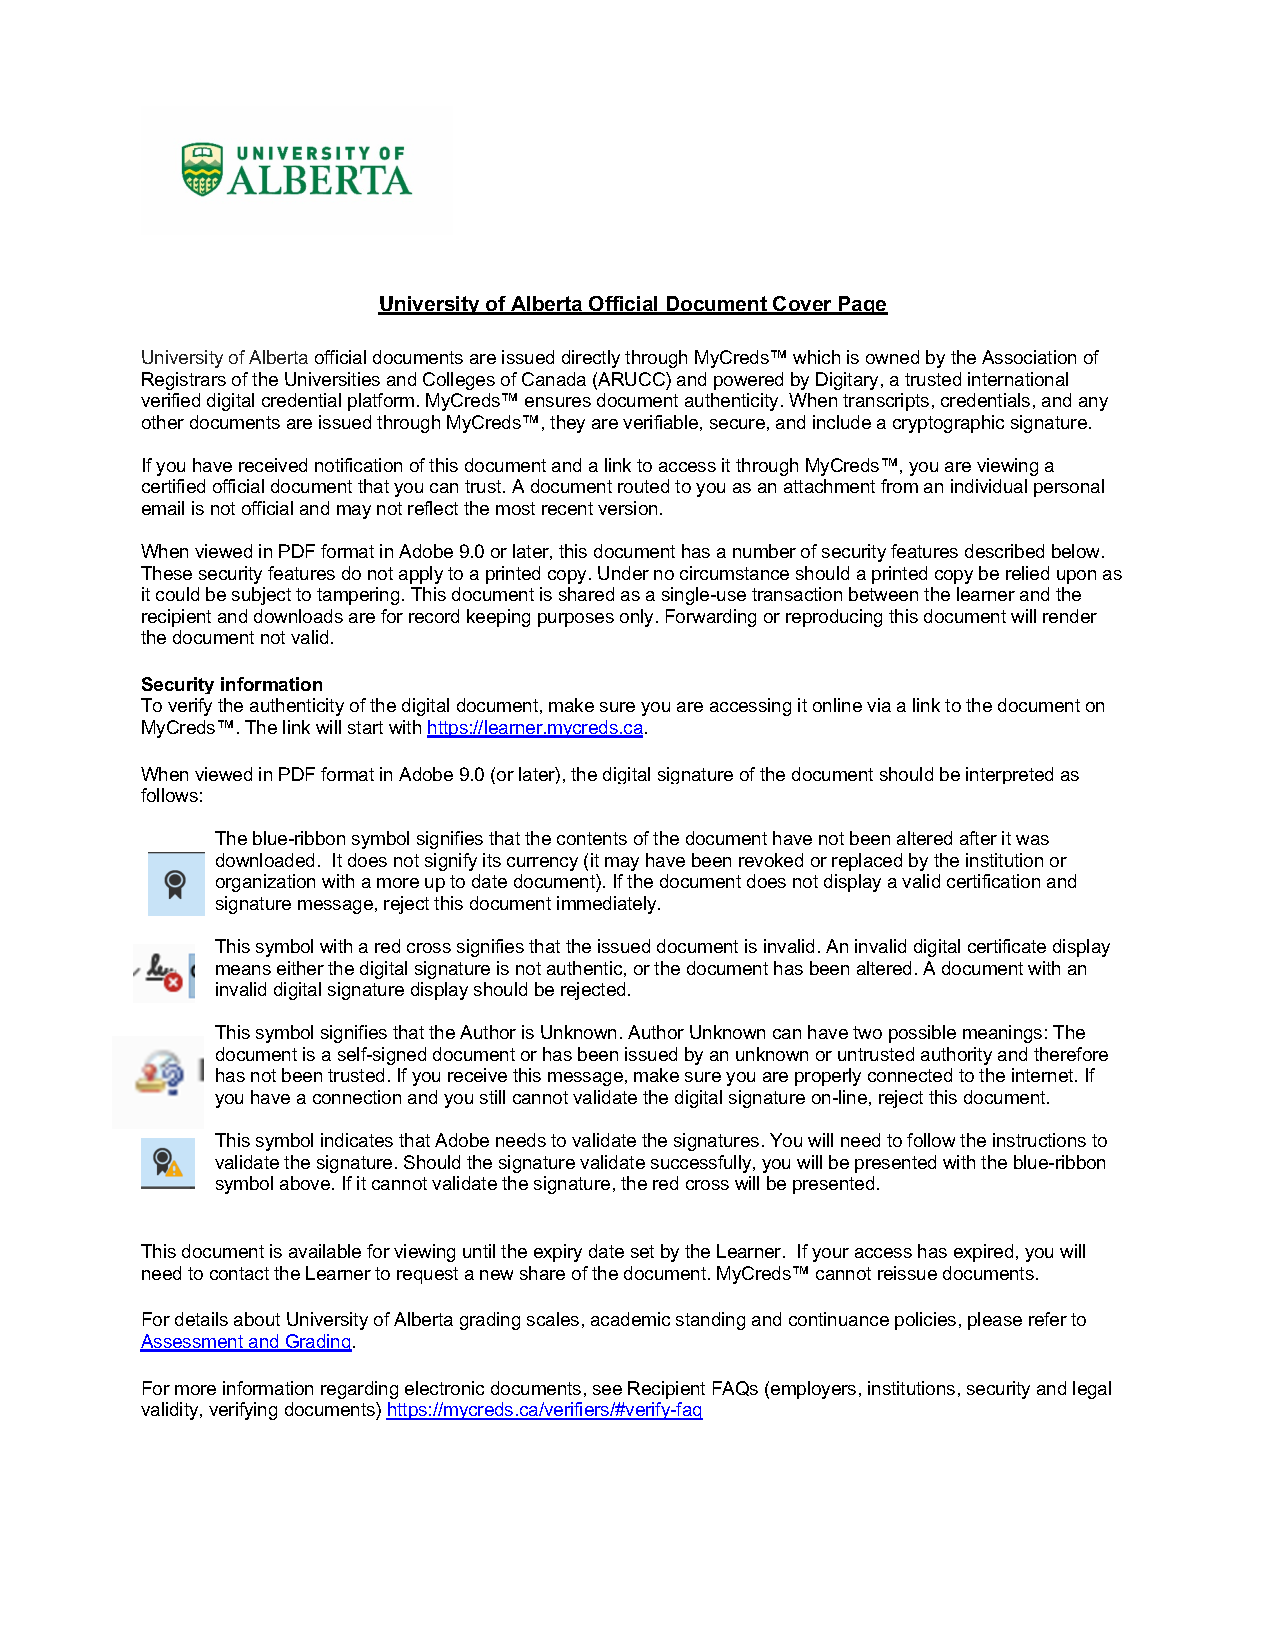
\includepdf[pages=-]{transcript}



    \section*{Correspondence about Graduation Certification}

    \includepdf[pages=-]{correspondence}



\end{document}